%%%%%%%%%%%%%%%%%%%%%%%%%%%%%%%%%%%%%%%%%
% APA Assignment Article
% LaTeX Template
% Version 2.0 (February 7, 2023)
%
% This template originates from:
% https://www.LaTeXTemplates.com
%
% Author:
% Vel (vel@latextemplates.com)
%
% License:
% CC BY-NC-SA 4.0 (https://creativecommons.org/licenses/by-nc-sa/4.0/)
%
% NOTE: The bibliography needs to be compiled using the biber engine.
%
%%%%%%%%%%%%%%%%%%%%%%%%%%%%%%%%%%%%%%%%%

%----------------------------------------------------------------------------------------
%	PACKAGES AND OTHER DOCUMENT CONFIGURATIONS
%----------------------------------------------------------------------------------------

\documentclass[
	letterpaper, % Paper size, use either a4paper or letterpaper
	10pt, % Default font size, can also use 11pt or 12pt, although this is not recommended
	unnumberedsections, % Comment to enable section numbering
	twoside, % Two side traditional mode where headers and footers change between odd and even pages, comment this option to make them fixed
]{APAAssignment}

\addbibresource{bibliography.bib} % BibLaTeX bibliography file

\runninghead{MICS CYBER 252, Fall-2024 Hands On Lab Unit 8} % A shortened article title to appear in the running head, leave this command empty for no running head

\footertext{\textit{Hands On Lab 8} (MICS CYBER 252, Fall -2024)} % Text to appear in the footer, leave this command empty for no footer text

\setcounter{page}{1} % The page number of the first page, set this to a higher number if the article is to be part of an issue or larger work

%----------------------------------------------------------------------------------------
%	TITLE SECTION
%----------------------------------------------------------------------------------------

\usepackage[title,toc,titletoc]{appendix}
\usepackage{titlesec}
\usepackage{lscape}
\usepackage{fontawesome}

\title{Hands On Lab: Unit 8 \\ MICS-252, Fall 2024 \\ Threat Analysis} % Article title, use manual lines breaks (\\) to beautify the layout

% Authors are listed in a comma-separated list with superscript numbers indicating affiliations
% \thanks{} is used for any text that should be placed in a footnote on the first page, such as the corresponding author's email, journal acceptance dates, a copyright/license notice, keywords, etc
% Affiliations are output in the \date{} command
\date{UC Berkeley School of Information \\
MICS Course 252 Fall 2024 (Kristy Westphal)
}


\author{
	Prepared by: Karl-Johan Westhoff \\
	email: \href{mailto:kjwesthoff@berkeley.edu}{kjwesthoff@berkeley.edu}
}


% % Full-width abstract
% \renewcommand{\maketitlehookd}{%
% 	\begin{abstract}
% 		\noindent Lorem ipsum dolor sit amet,rta porttitor.
% 	\end{abstract}
% }

%----------------------------------------------------------------------------------------

\setcounter{tocdepth}{5}
\setcounter{secnumdepth}{5}
\usepackage[title]{appendix}

\begin{document}
\onecolumn
\maketitle % Output the title section

%----------------------------------------------------------------------------------------
%	ARTICLE CONTENTS
%----------------------------------------------------------------------------------------


\section{Introduction}
Threat intelligence is when an adversary is associated with the data. To better understand adversaries and how to account for them in threat modeling, it is useful to put adversaries into categories defined by what they want, what their capabilities are, and how they conduct their 'activities'\footnote{Tactics Techniques and Procedures (TTP), "modus operandi" in classic spy terms} in this assignment I decided to look at threat actors who target cloud 'systems', many 'things' are moving/have moved to the cloud\footnote{A 'reaction' going in the opposite direction, in-sourcing and self-hosting is also occurring\cite{DHH_leftTheCloud}}. Cloud-ification offers security benefits:
\begin{itemize}
	\item Someone else handles security often with synergies doing it for many customers
	\item Increased reliability, and availability etc.
\end{itemize}

But is also comes with a significant problem:
\begin{itemize}
	\item Someone else is handling your security
\end{itemize}

With a 'someone else' is handling parts of your security as a part of their hosting service, there is a risk for responsibilities "falling between two stools", especially in complicated architectures with services from different cloud systems. This often makes enterprises terrible at security \cite{CloudComputingInsider} defines a "toxic cloud triad" of highly privileged, publicly exposed workloads with weak configuration. The adversaries know this and targets default configuration and especially access control to breach and achieve persistence on cloud systems.

\section{Scattered Spider}
\subsection{Description}
According to MITRE\cite{MITRE_ScatteredSpider} Scattered Spider has been active since 2022, and initially targeted customer relations systems and telecommunication companies. Apparently they figured out that they were good at obtaining credentials to systems using social engineering. They did this by portraying to be employees or internal IT often in longer duration social engineering acts, Hence MITRE concluded that they are native English speakers. Crowdstrike included a section on Scattered Spider in their 2024 Global Threat Report \cite{CrowdStrikeGTR2024}, shown in Appendix \ref{app:CrowdStrikeScatteredSpider} and describes their modus of targeting IT services using elaborate social engineering.

\subsection{Targets}
CISA\cite{CISA_ScattetedSpider} has defined Scattered Spider as a cyber criminal group targeting information systems of large companies for extortion. \\
Most notably the group targeted the "MGM Grand" casino resort, the attack was carried out in 'joint venture'\footnote{This has neither been confirmed nor denied by either parties} with "ALPHV/BlackCat"\cite{UHonMGM-ALPHV}\cite{VOXonMGM-Hack}, providing "Ransomware as a service"\footnote{This whole hacker thing is increasingly becoming corporate}. The attack disrupted operations for 10 days ,they had to shut down systems and operate 'manually', notify their customers and cost MGM \$100M\cite{UHonMGM-ALPHV}, but who knows - what happens in Vegas stays in Vegas.

\subsubsection{Targets summary:} Larger corporations for extortion

\subsection{Modus Operandi}
Scattered Spider are able to conduct elaborate social engineering campaigns, using open intelligence (LinkedIn etc.) to circumvent security measures (see quote in Appendix \ref{app:voxSocialEngQuote}). Furthermore they are able to leverage deep knowledge on various cloud systems (Azure Active Directory) and identity management (OKTA) get a foothold. From there various tools for monitoring and ex filtration (Fleetdeck etc.), credential extraction (e.g. Mimikatz) and malware (eg. ransomware) are deployed. CISA has compiled a list based on MITRE Att\&ck in \cite{CISA_ScattetedSpider} and depicted in Appendix \ref{app:SoftwareTools}. \\

\subsubsection{The MGM attack} \cite{UHonMGM-ALPHV} has a good write-up on how Scattered Spider gained initial foothold.

\begin{enumerate}
	\item Use OSint (LinkedIn etc.) to identify a suitable employee and assume their identity
	\item Call MGM IT requesting assistance to log in
	\item A 10 minute phone call allegedly gave administrator privileges to MGM OKTA and Azure environments even with MFM in place (using phone sim hijacking)
	\item Deploy reconnaissance and terminate security software (POORTRY/STONESTOP see Appendix \ref{app:DetectionAvoidance})\cite{TrellixScattetedSpider}
	\item Deploy command and control for persistence and ex-filtration
\end{enumerate}

\subsubsection{Modus Operandi Summary} Use knowledge of systems and elaborate social engineering (voice phishing, "vishing") and advanced techniques  (sim hijacking) to convince victim to provide credentials (even when these are multi factor (MFA))

\subsection{TTP's}
CISA article \cite{CISA_ScattetedSpider} Has a detailed set of tables with the MITRE att\&ck Tactics and Techniques a condensed summary there of is :
\begin{itemize}
	\item Reconnaissance:
	      \begin{itemize}
		      \item Gather victim identities using SoMe profiles
		      \item Gather information in victim system/architecture
	      \end{itemize}
	\item Resource Development
	      \begin{itemize}
		      \item Fake SoMe accounts to back up phishing stories
		      \item Establish ephemeral domains
		      \item Phone SIM hijacking, number stealing
	      \end{itemize}
	\item Initial Access, using 'Social Engineering'
	      \begin{itemize}
		      \item Phishing targeted against IT access control, either posing as IT asking for credentials, or posing as employees requesting MFA reset etc.
		      \item Elaborate, convincing phone voice phishing 'acts' (Vishing), fluent in English
		      \item SMS phishing using hijacked numbers to convince credentials handover (smishing)
		      \item MFA fatigue (someone accepting after receiving many MFA approval notifications)
	      \end{itemize}
	\item Execution, Persistence, Privilege Escalation, Defense Evation
	      \begin{itemize}
		      \item Collect data, credentials etc. using e.g Mimikatz see Appendix \ref{app:SoftwareTools}
		      \item Impersonate IT gain remote desktop access (again requiring social skills to be convincing)
		      \item Create new users
	      \end{itemize}
	\item Extortion and data theft
	      \begin{itemize}
		      \item Establish C2 infrastructure
		      \item Gather, compress and ex filtrate data
		      \item Start extortion campaign
	      \end{itemize}
\end{itemize}
\subsection{Recommendations}



\section{Conclusion}
I'm not so sure they can keep the vishing campaigns up, the use of their voice gives possibility for profiling and subsequent attribution



\section{Notes}
Include how the group typically targets, the methods that they use, and what their typical goal is.

1. Begin by choosing a threat actor group from the MITRE page.\\
2. Utilizing open source intelligence, research who the group typically targets, what methods they use to attack their targets and what they are generally after.\\
3.Identify any known tactics, techniques and procedures.\\
4. Make recommendations on actions that a SOC can take with the data that you have found on your chosen threat group. \\
5. Be sure to document all of the sources that you utilize in your research. \\


\section{Notes}
The one size fits all for cloud security means that the same holes are found in many walls. This can be utilized to get a foothold in many locations using the same methodology.











%\begin{figure}[!htp] % Single column :figure	
%	\centering
% 	\includegraphics[width=0.5\linewidth]{STRIDE.png}
% 	\caption{The STRIDE model summarized, illustration from \cite{STRIDE_For_pay_Medium}}
% 	\label{fig:STRIDE}
% \end{figure}
%

%----------------------------------------------------------------------------------------
%	 REFERENCES
%----------------------------------------------------------------------------------------

\printbibliography % Output the bibliography

%----------------------------------------------------------------------------------------



%----------------------------------------------------------------------------------------
%	 Appendices
%----------------------------------------------------------------------------------------

\appendix


\clearpage
\chapter{Appendices}
\begin{appendices}
	\section{Scattered Spider Section from Crowdstrike's 2024 Report}\label{app:CrowdStrikeScatteredSpider}

	\begin{figure}[!htp] % Single column :figure	
		\centering
		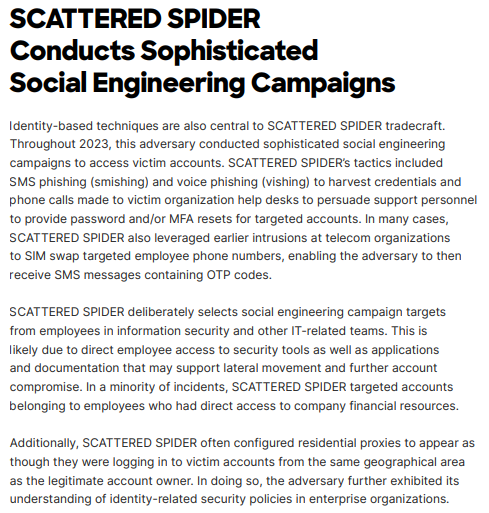
\includegraphics[width=0.75\linewidth]{CrowdstrikeScatteredSpider.png}
		\caption{Crowdstrike, Global Threat Report 2024, Scattered spider section from \cite{CrowdStrikeGTR2024}}
		\label{fig:CrowdStrikeScatteredSpider}
	\end{figure}

	\section{Comment on the MGM attacks and 'vishing' modus}\label{app:voxSocialEngQuote}
	CISO's comment on the use of social engineering in the MGM attack, from VOX\cite{VOXonMGM-Hack}: \\
	"There’s always a little back door, and all the best defenses and all the expensive tools can be fooled by one good social engineering attack,” Peter Nicoletti, global chief information security officer at cybersecurity company Check Point Software, told Vox.

	\section{CISA compiled list of soft/malware tools}\label{app:SoftwareTools}

	\begin{figure}[!htp] % Single column :figure	
		\centering
		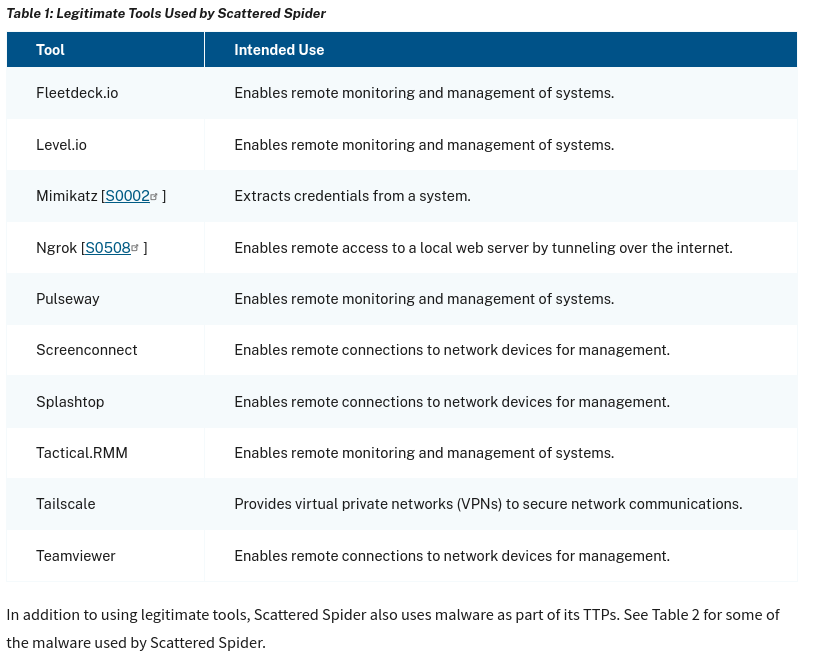
\includegraphics[width=0.75\linewidth]{CISATools1.png}
		\caption{'Legitimate' software tools used by Scattered Spider\cite{CISA_ScattetedSpider}}
		\label{fig:CISATools1}
	\end{figure}

	\begin{figure}[!htp] % Single column :figure	
		\centering
		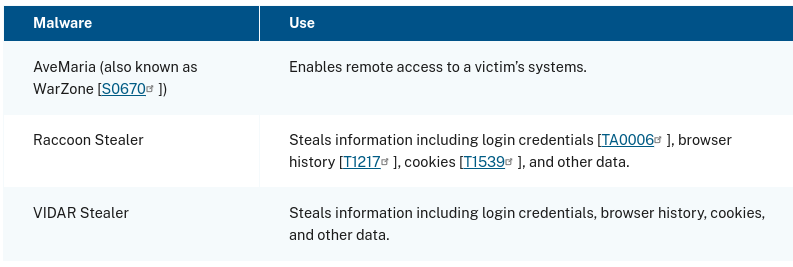
\includegraphics[width=0.75\linewidth]{CISATools2.png}
		\caption{'Malware' tools used by Scattered Spider\cite{CISA_ScattetedSpider}}
		\label{fig:CISATools2}
	\end{figure}

	\section{Tools used to evade detection}\label{app:DetectionAvoidance}
	Scattered Spider typically exploits vulnerabilities such as CVE-2015-2291 \cite{TrellixScattetedSpider}
	\begin{itemize}
		\item{POORTRY is a malicious driver used to terminate selected processes on Windows systems, e.g., Endpoint Detection and Response (EDR) agent on an endpoint.11 To evade detection, attackers have signed POORTRY driver with a Microsoft Windows Hardware Compatibility Authenticode signature.}
		\item{STONESTOP is a Windows userland utility that attempts to terminate processes by creating and loading a malicious driver.13 It functions as both a loader/installer for POORTRY, as well as an orchestrator to instruct the driver with what actions to perform}
	\end{itemize}



\end{appendices}
\end{document}
